\documentclass[aspectratio=169]{beamer}

% Compile with pdfLaTeX.
\usepackage[T2A]{fontenc}
\usepackage[utf8]{inputenc}
\usepackage[russian,english]{babel}
\usepackage{graphicx}
\usepackage[defaultsans]{opensans}
\usepackage{tabularx}
\usefonttheme{professionalfonts}
\renewcommand{\familydefault}{\sfdefault}

\setbeamercolor{normal text}{fg=black}
\setbeamercolor{structure}{fg=black}
\setbeamercolor{frametitle}{fg=black}
\setbeamercolor{footline}{fg=black}
\setbeamercolor{item}{fg=black}
\setbeamercolor{subitem}{fg=black}
\setbeamercolor{subsubitem}{fg=black}
\setbeamercolor{title}{fg=white}

\setbeamerfont{normal text}{family*=\opensansfamily}
\setbeamerfont{title}{family*=\opensansfamily,size=\Huge,series=\bfseries}
\setbeamerfont{frametitle}{family*=\opensansfamily,series=\bfseries}
\setbeamerfont{footline}{family*=\opensansfamily}
\setbeamerfont{author}{family*=\opensansfamily}
\setbeamerfont{date}{family*=\opensansfamily}
\setbeamerfont{institute}{family*=\opensansfamily}

\setbeamertemplate{navigation symbols}{}
\setbeamertemplate{footline}[frame number]
\setbeamertemplate{frametitle}{%
  \vspace*{0.5cm}
  \nointerlineskip
  \begin{beamercolorbox}[wd=\paperwidth,ht=2.8ex,dp=1.1ex,leftskip=5.7cm]{frametitle}
    \usebeamerfont{frametitle}\insertframetitle
  \end{beamercolorbox}%
}

\vspace*{1cm}
\title{Распознавание рукописного текста с анализом эмоциональной окраски}
\date{}

\newcommand{\slidebg}[1]{%
  \setbeamertemplate{background}{%
    \parbox[c][\paperheight][c]{\paperwidth}{%
      \includegraphics[width=\paperwidth,height=\paperheight]{#1}%
    }%
  }%
}

\begin{document}


\slidebg{assets/1.png}
\begin{frame}[plain,noframenumbering]
  \titlepage
\end{frame}


\slidebg{assets/2.png}
\begin{frame}
  \frametitle{Актуальность}
  \begin{itemize}
    \item Цифровизация рукописных архивов и исторических документов.
    \item Снижение ручного труда при вводе текстов из бумажных источников.
    \item Сокращение числа ошибок и времени обработки данных.
    \item Применение в образовании, медицине и документообороте.
    \item Основа для последующего анализа содержания и тональности текста.
  \end{itemize}
\end{frame}

\slidebg{assets/2.png}
\begin{frame}
  \frametitle{Пример готового решения}
   \begin{center}
    \hspace*{-2.9cm}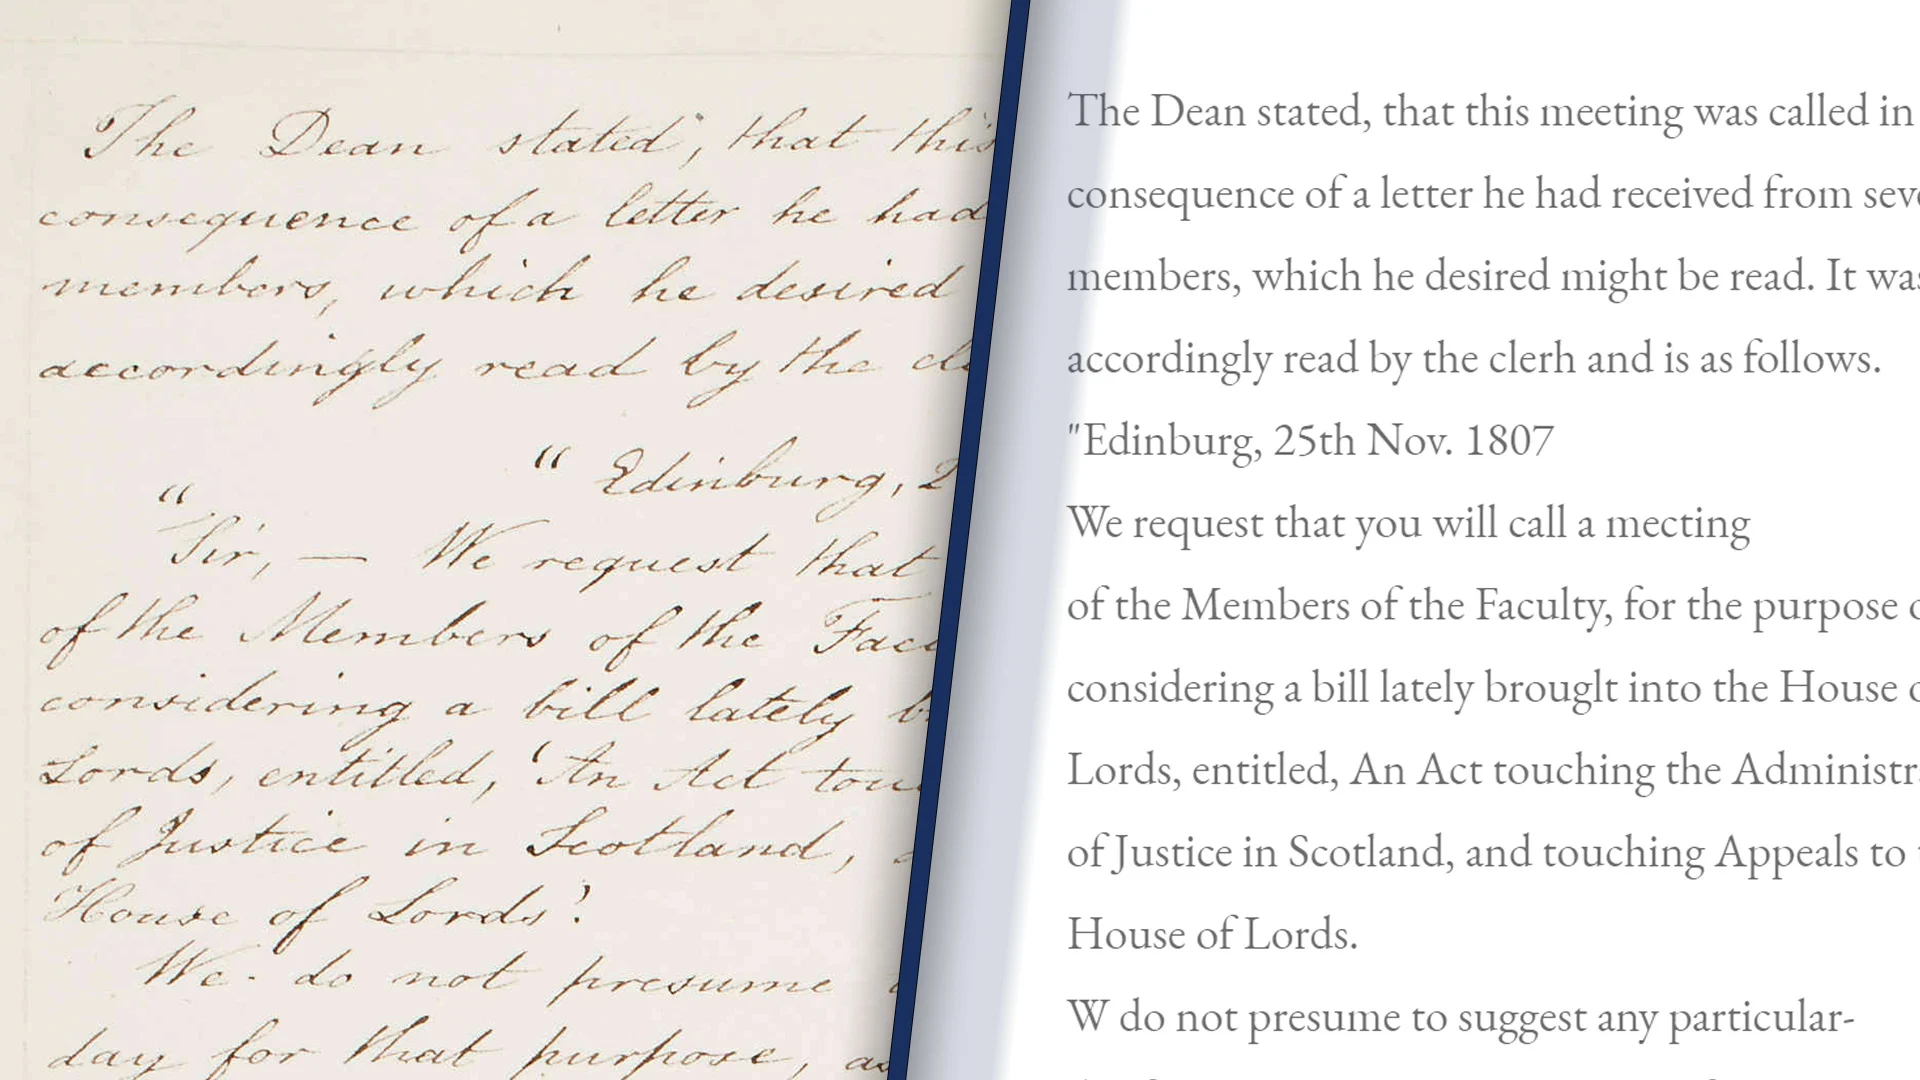
\includegraphics[width=1\textwidth,height=0.8\textheight,keepaspectratio]{assets/hwr_example_1.png}
  \end{center}
\end{frame}

\slidebg{assets/2.png}
\begin{frame}
  \frametitle{Цель и задачи работы}
  \scriptsize
  \textbf{Цель работы:} разработать программный инструмент для автоматического распознавания рукописного текста и последующего анализа тональности распознанного содержания.

  \vspace{0.3em}
  \textbf{Задачи работы:}
  \begin{columns}[T,onlytextwidth]
    \begin{column}{0.49\textwidth}
      \begin{itemize}
        \setlength{\itemsep}{0.2em}
        \item Проанализировать существующие подходы к распознаванию рукописного текста и анализу тональности.
        \item Подобрать и подготовить датасет для обучения и тестирования модели.
        \item Определить метрики качества и критерии успешности решения.
        \item Разработать и реализовать модель распознавания рукописного текста.
      \end{itemize}
    \end{column}
    \begin{column}{0.49\textwidth}
      \begin{itemize}
        \setlength{\itemsep}{0.2em}
        \item Обучить модель и оценить качество её работы на выбранном датасете.
        \item Реализовать модуль анализа тональности распознанного текста.
        \item Объединить распознавание и анализ тональности в единый программный инструмент.
      \end{itemize}
    \end{column}
  \end{columns}
\end{frame}

\slidebg{assets/2.png}
\begin{frame}
  \frametitle{Подходы к распознаванию: плюсы и минусы}
  \scriptsize
  \setlength{\tabcolsep}{4pt}
  \renewcommand{\arraystretch}{1.15}
  \begin{tabularx}{\textwidth}{|X|X|X|X|}
    \hline
    \textbf{Подход} & \textbf{Плюсы} & \textbf{Минусы} & \textbf{Где лучше работает} \\
    \hline
    Классический OCR (правила, сегментация) & Простота, низкие требования к ресурсам & Плохо переносит сложный почерк и шум & Печатный или аккуратный текст \\
    \hline
    CRNN + CTC & Не нужна посимвольная разметка, устойчив к разной длине строк, сильный базовый результат & Чувствителен к качеству предобработки, требует обучения & Рукописные строки средней сложности \\
    \hline
    Transformer-подходы (TrOCR и аналоги) & Высокий потенциал качества, гибкость архитектуры & Высокая вычислительная стоимость, сложнее обучение & Большие датасеты и мощные вычисления \\
    \hline
  \end{tabularx}

  \vfill
  \textbf{Анализ показал, что наиболее результативным является метод CRNN + CTC.}
\end{frame}


\slidebg{assets/2.png}
\begin{frame}
  \frametitle{Последовательность этапов решения}
  \begin{itemize}
    \item Подготовка данных: очистка, выравнивание, нормализация.
    \item Разбиение выборки на обучающую, валидационную и тестовую части.
    \item Препроцессинг изображений, аугментация обучающей выборки.
    \item Нормализация пакетов данных для подачи в модель.
    \item Обучение сверточной рекуррентной нейронной сети с использованием CTC-loss.
    \item Декодирование выходов модели в текстовую форму.
    \item Оценка качества на валидационной и тестовой выборках.
    \item Интеграция модуля анализа тональности распознанного текста.
  \end{itemize}
\end{frame}


\slidebg{assets/2.png}
\begin{frame}
  \frametitle{Подготовка данных}
  \begin{columns}[T,onlytextwidth]
    \begin{column}{0.58\textwidth}
      \begin{itemize}
        \item Для обучения модели будет использоваться датасет IAM Handwriting Database, который содержит рукописные тексты с разметкой.
        \item Датасет включает в себя изображения строк рукописного текста и соответствующие им текстовые транскрипты.
      \end{itemize}
    \end{column}
    \begin{column}{0.38\textwidth}
      \centering
      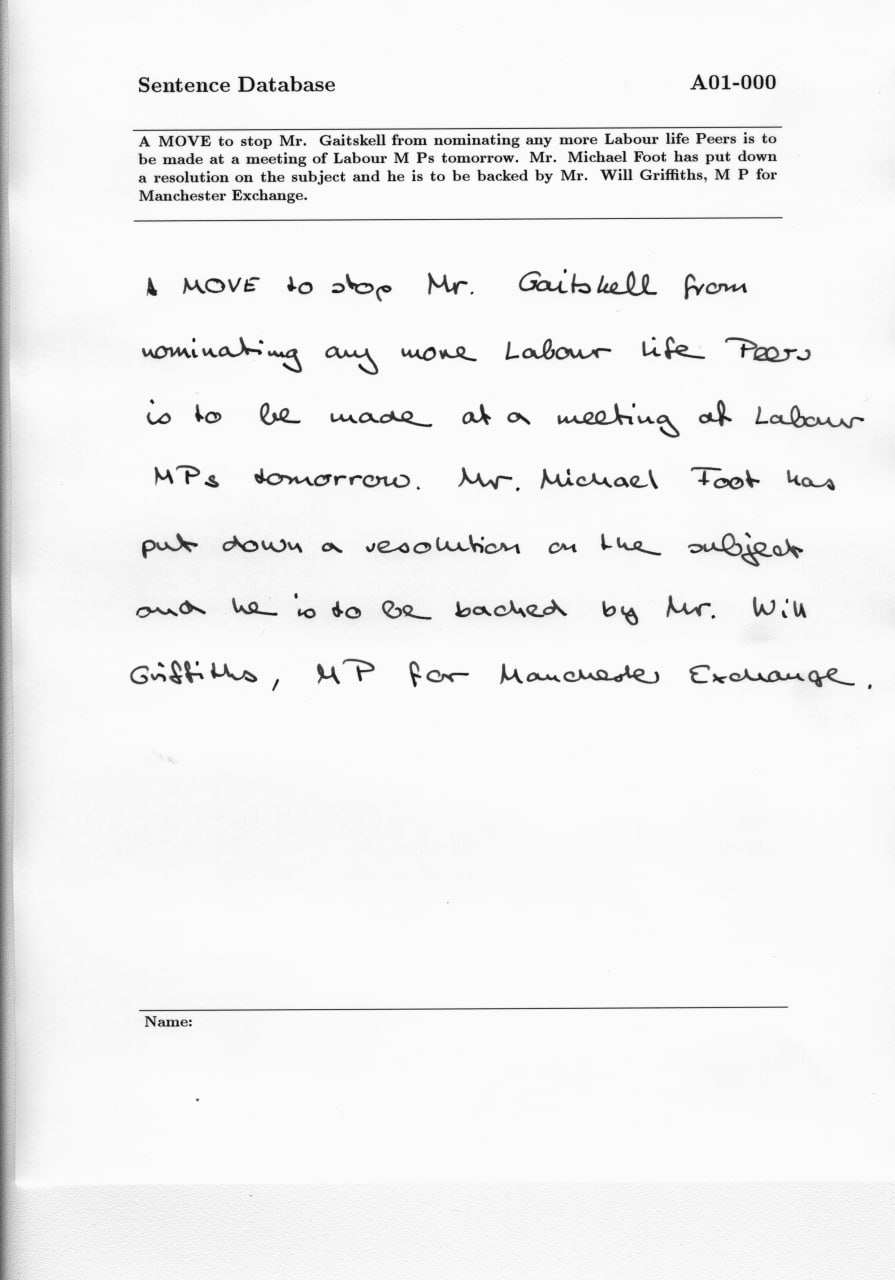
\includegraphics[width=\linewidth,height=0.8\textheight,keepaspectratio]{assets/iam_3.jpeg}
    \end{column}
  \end{columns}
\end{frame}


\slidebg{assets/2.png}
\begin{frame}
  \frametitle{Разбиение выборки}
  \begin{itemize}
    \item Датасет будет разделен на обучающую, валидационную и тестовую части в соотношении 70\% - 15\% - 15\%.
    \item Важно обеспечить, чтобы строки из одного документа не попадали одновременно в разные части выборки, чтобы избежать утечки данных.
    \item Строки одного автора также будут распределены по разным частям выборки, чтобы модель не могла просто запомнить почерк конкретного человека.
  \end{itemize}
\end{frame}


\slidebg{assets/2.png}
\begin{frame}
  \frametitle{Препроцессинг изображений}
  \begin{center}
    \hspace*{-0.55cm}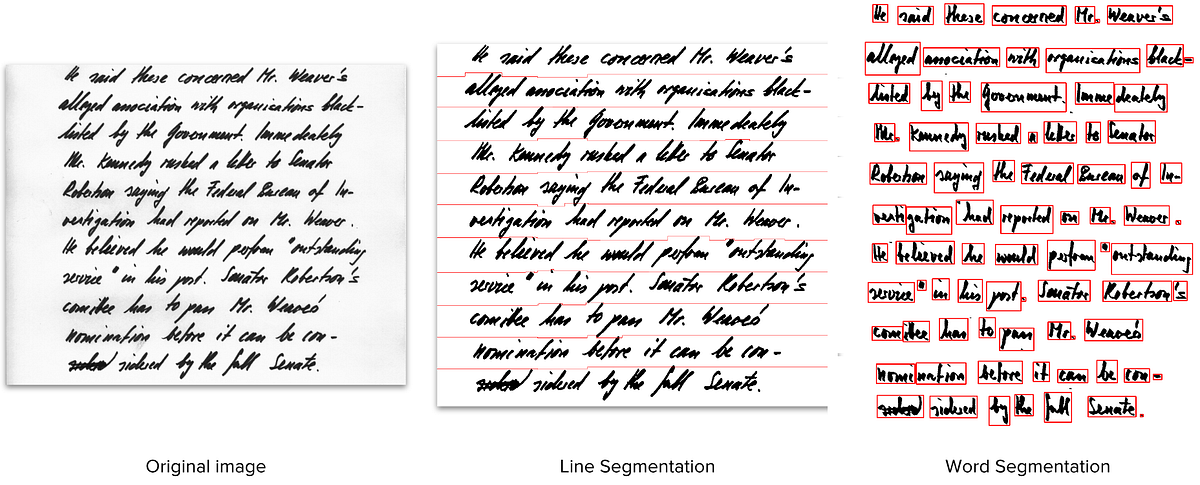
\includegraphics[width=1.08\textwidth,height=1.05\textheight,keepaspectratio]{assets/segmentation_1.png}
  \end{center}
\end{frame}



\slidebg{assets/2.png}
\begin{frame}
  \frametitle{Сверточная нейронная сеть}
Сверточные нейронные сети (CNN) - разновидность нейронных сетей. Часто используется в задачах компьютерного зрения.

Кратко про последовательность работы:

\begin{itemize}
    \item Входное изображение представляется в виде матрицы - \(P_{n \times n}\)
    \item По изображению последовательно применяются свертки с помощью ядра - матрицы \(C_{k \times k}, k \ll n\)
    \item Свертка - процесс перемножения ядра свертки и области изображения, на которую оно наложено, с последующим суммированием результатов.
    % \item Результат свертки - новая матрица признаков, которая содержит информацию о локальных особенностях изображения, таких как края, текстуры и формы.
\end{itemize}

\end{frame}

\slidebg{assets/2.png}
\begin{frame}
  \frametitle{CRNN: визуализация}
  \begin{center}
    \hspace*{-2.9cm}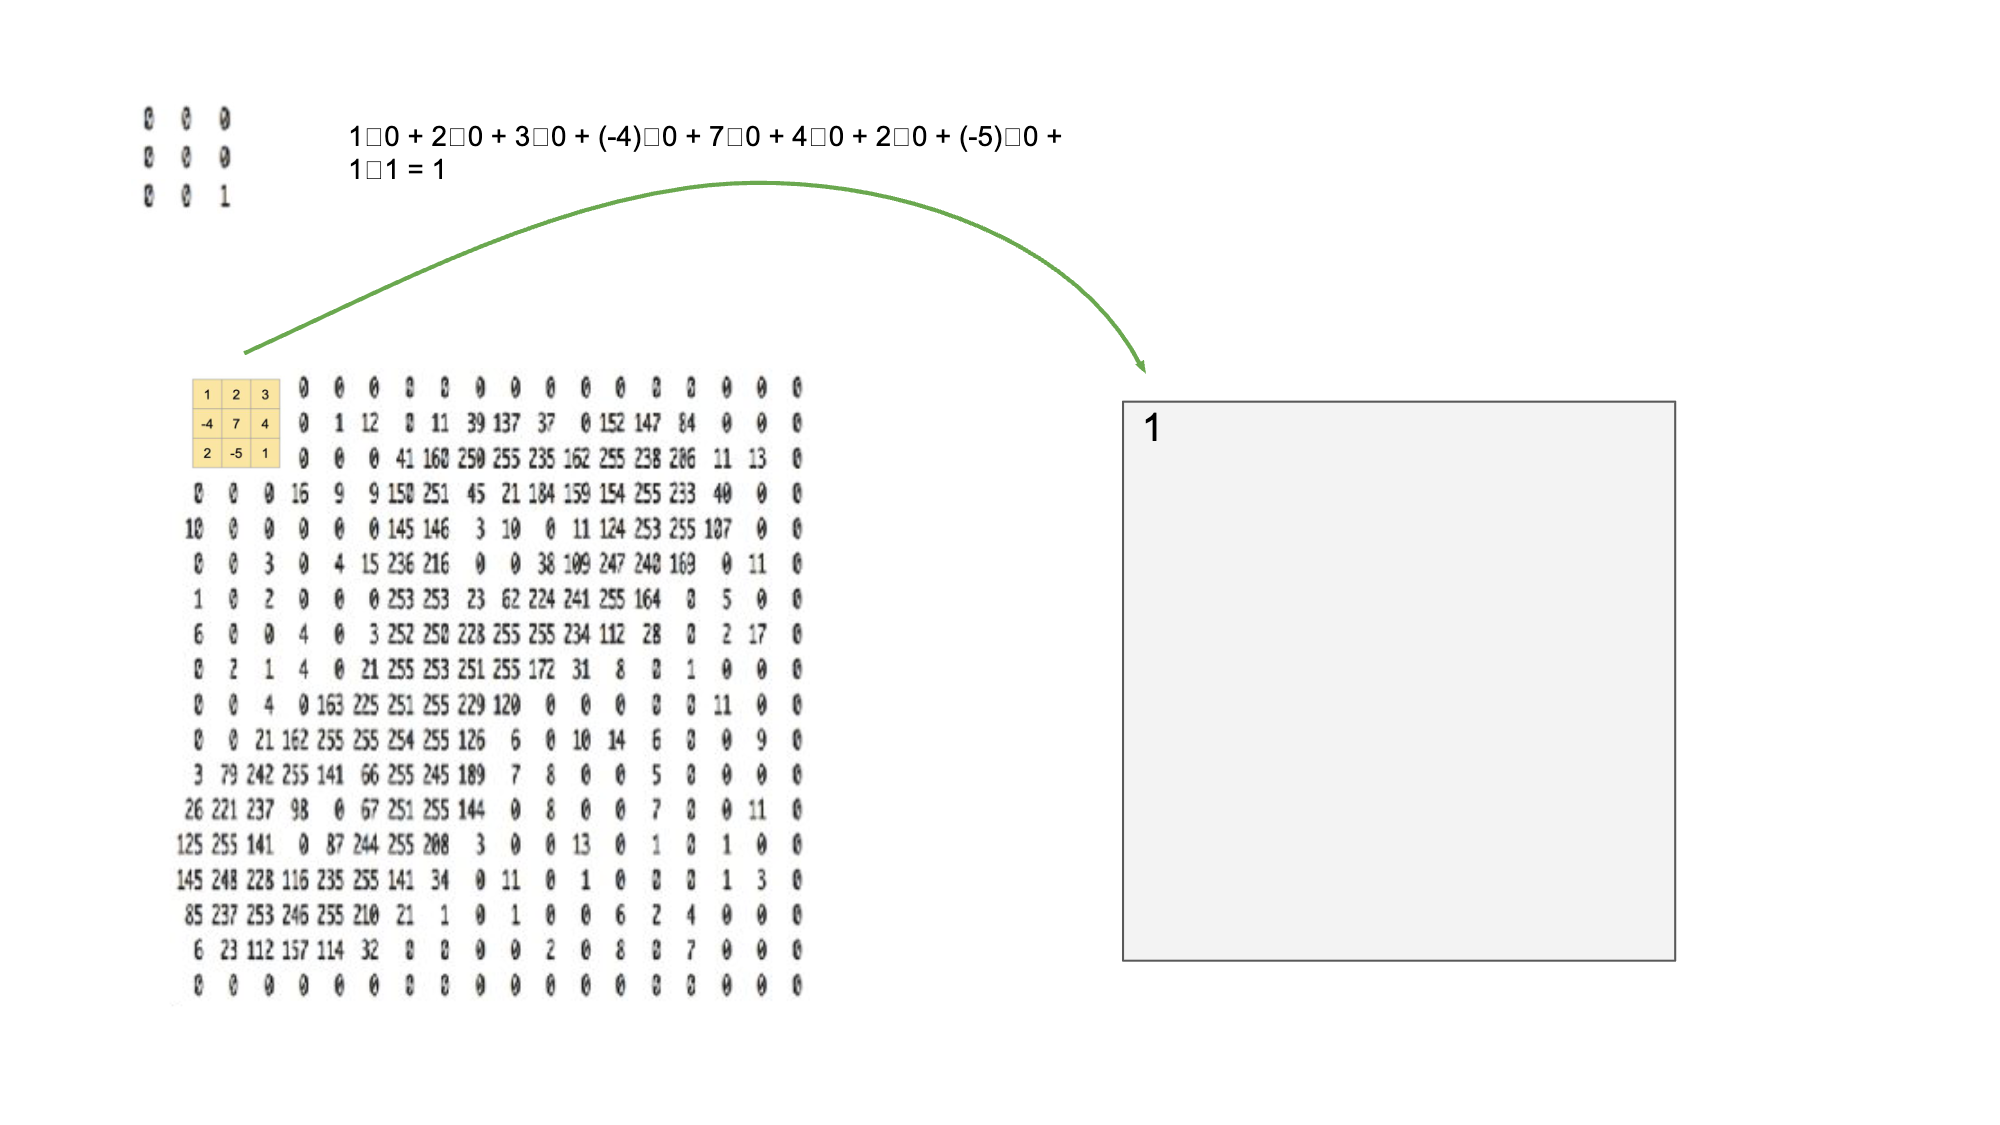
\includegraphics[width=1\textwidth,height=0.8\textheight,keepaspectratio]{assets/CRNN_visualisation.png}
  \end{center}
\end{frame}

\slidebg{assets/2.png}
\begin{frame}
  \frametitle{CRNN: визуализация}
  \begin{center}
    \hspace*{-2.9cm}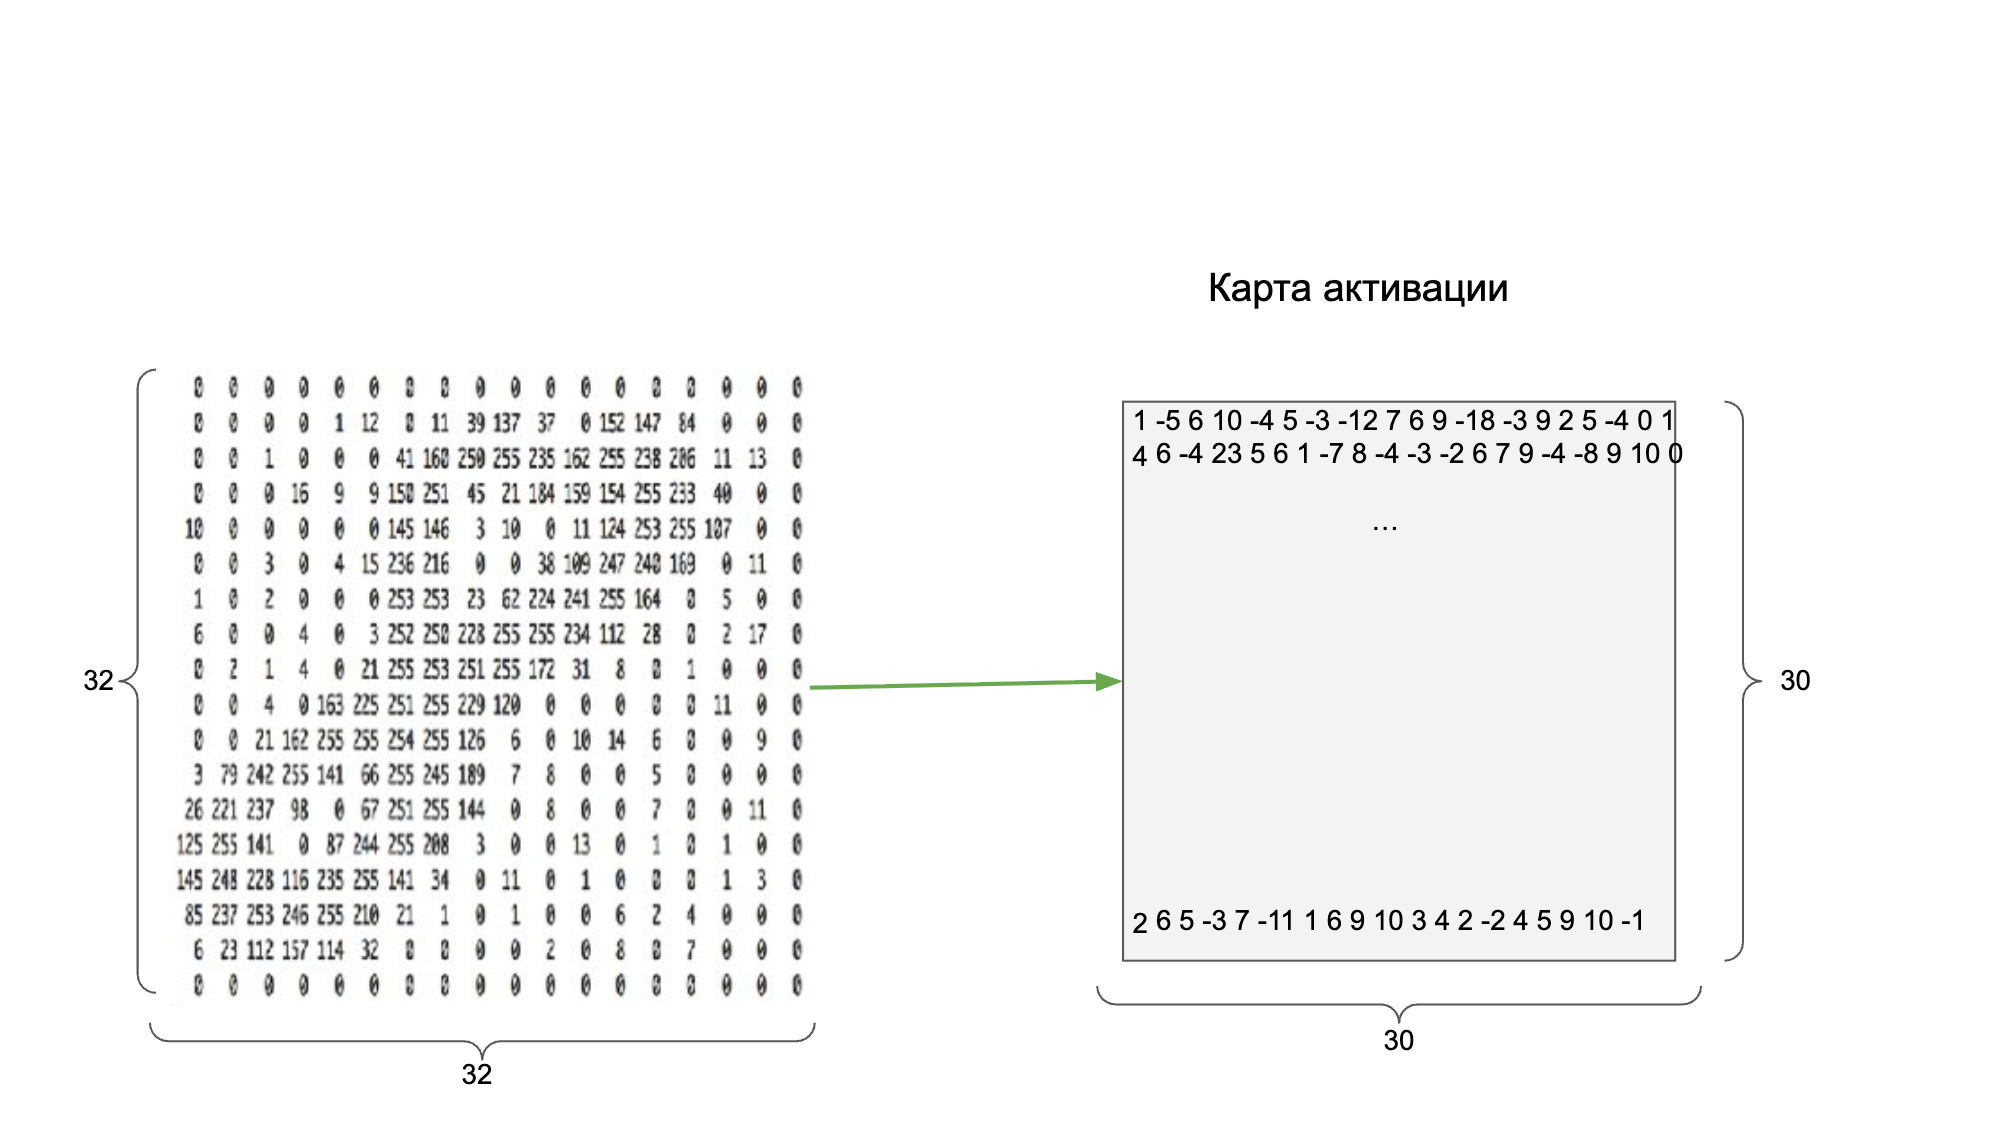
\includegraphics[width=1\textwidth,height=0.8\textheight,keepaspectratio]{assets/CRNN_2.png}
  \end{center}
\end{frame}

\slidebg{assets/2.png}
\begin{frame}
  \frametitle{Сверточная нейронная сеть}
  \begin{itemize}
    \item Результат свертки - новая матрица признаков - \(\mathbf{P}_{n-k+1 \times n-k+1}\)
    \item Высокие значения указывают на участки изображения, которые соответствуют шаблону, задаваемому ядром свертки. Низкие значения указывают на отсутствие такого шаблона.
    \item Свертки позволяют модели учиться распознавать сложные шаблоны и структуры в изображении, что особенно важно для задач распознавания рукописного текста, где могут быть вариации в почерке, наклоне и размере символов.
    \item Полученная матрица признаков в виде вектора подается на вход полносвязной нейронной сети.
  \end{itemize}
\end{frame}

\slidebg{assets/2.png}
\begin{frame}
  \frametitle{Метрики качества}
  \begin{itemize}
    \item \textbf{CER (Character Error Rate)} \(= \frac{\text{количество ошибок}}{\text{общее количество символов}}\). Метрика, которая измеряет количество ошибок в распознанном тексте.
    \item \textbf{WER (Word Error Rate)} \(= \frac{\text{количество ошибок}}{\text{общее количество слов}}\). Метрика, которая измеряет количество ошибок в распознанных словах.
  \end{itemize}
  Ошибки - вставки, удаления и замены символов или слов. Чем ниже эти метрики, тем лучше качество распознавания.
\end{frame}

\slidebg{assets/2.png}
\begin{frame}
  \frametitle{Метрики: пример}
Истинный текст: \texttt{The quick brown fox jumps over the lazy dog.}

Распознанный текст: \texttt{The \textcolor{red}{qucik} brown fox \textcolor{red}{jumpts} \textcolor{red}{ove} the lazy \textcolor{red}{do}.}
  \begin{itemize}
    \item Количество символов: $44$ (включая пробел)
    \item Ошибки: $4$ (вставка, удаление, замена)
    \item CER = \((4 / 44) * 100 = 9.09\%\)
  \end{itemize}
  \begin{itemize}
    \item Количество слов с ошибками: $4$ (\texttt{qucik, jumpts, ove, do})
    \item Количество слов: $9$
    \item WER = \((4 / 9) * 100 = 44.44\%\)
  \end{itemize}
\end{frame}

\slidebg{assets/3.png}
\begin{frame}
  \centering
  \Huge Спасибо за внимание!
\end{frame}

\end{document}
